\section{Collision Detection}
\label{sec:chapter_navigazione_scena_collision_detec}

Per collision detection si intende il problema di determinare l’intersezione tra due o più oggetti. 
\\
In particolare è necessario determinare quando e dove i due oggetti sono stati intersecati stabilendo in quale momento ed in quale punto, durante il movimento, la collisione è avvenuta.
\\
La collision detection viene utilizzata in varie applicazioni come videogiochi, simulazioni basate sulla fisica (come le animazioni grafiche) e robotica.
\\
In questo lavoro di tesi è stata utilizzata nel navigatore per fornire all’utente l’illusione di aver creato una scena solida.
\\
La collision detection viene infatti attivata quando vengono abilitati i controlli in prima persona e permette durante la navigazione della scena di simulare il comportamento reale di una persona che cammina dentro un appartamento.
\\
La gestione delle collisioni permette all’osservatore virtuale pilotato dall’utente di saltare e, quando possibile, salire o scendere (es: salire le scale). Inoltre ha permesso di bloccare i movimenti di navigazione nel caso di attraversamento di oggetti o muri.
\\
L’algoritmo che permette le collisioni incide pesantemente sulle performance real-time.
Questi algoritmi effettuano normalmente effettuano un enorme quantitativo di query e calcoli delle collisioni per ogni frame. 
\\
Questi calcoli si aggiungono a quelli già effettuati dal rendering comportando un incremento del carico di lavoro della CPU con conseguente diminuzione degli fps generali. Un algoritmo di questo tipo può infatti facilmente diventare un collo di bottiglia anche con un basso numero di oggetti da renderizzare.
\\
Se infatti all’interno di una scena sono presenti n oggetti in cui ogni oggetto può potenzialmente collidere con gli altri, è necessario effettuare il test di collisione tra ogni coppia di oggetti presenti. 
\\
Si ottiene in questo modo un algoritmo di complessità quadratica  dipendente dal numero di oggetti nella scena:
\begin{equation}
(n - 1) + (n - 2) ... + 1 = \frac{n(n - 1)}{2} = \mathcal{O}^2
\end{equation}
Come intuibile, effettuare il test su ogni coppia risulta impraticabile in ambienti browser in quanto rallenterebbe troppo il servizio di navigazione. 
\\
In questo lavoro di tesi è stato quindi essenziale l’ implementazione di un algoritmo che permettesse di diminuire il numero di test di collisione da effettuare, in maniera tale da risultare efficiente in applicazioni real-time su web.
\\
Per la creazione dell’algoritmo è stato necessario analizzare il contesto preso in esame da questo elaborato.
La navigazione in prima persona viene effettuata su una scena su cui è stato applicato il processo di bake e quindi una scena statica. Siccome la scena risulta immodificabile nel tempo, è impossibile che gli oggetti presenti in essa possano collidere in quanto immobili.
Solamente l’osservatore virtuale si muove all’interno della scena e quindi è l’unico che può collidere con l’ambiente.
\\
Di fatto quindi risulta inutile effettuare il test di collisione per ogni coppia di oggetti presenti nella scena, per questo viene effettuato per ogni coppia (osservatore, oggetto x), dove x= 1...n.
\\
Questo ha permesso di velocizzare l’algoritmo, permettendo di far scendere la complessità da quadratica a lineare.
\\
Viene inoltre ottimizzato ulteriormente l’algoritmo di collisione effettuando una separazione della collisione in due fasi: una fase generale (\texttt{broad phase}) ed una fase ristretta (\texttt{narrow phases}) \cite{real_time_collision}.
\\
La fase generale identifica dei piccoli gruppi di oggetti che potrebbero collidere e esclude velocemente quelli che non potrebbero.
\\
La fase ristretta effettua il test di collisione solamente sulle coppie dei piccoli gruppi identificati nella fase precedente.
\\
Questa strategia dividi e conquista ha permesso di ottenere un enorme miglioramento delle prestazioni dell’algoritmo e dell’applicazione navigatore in generale. Queste due fasi saranno dettagliate nei due paragrafi seguenti.

\subsection{Fase generale}
La fase generale dell’algoritmo di collision detection permette di individuare le coppie di oggetti rigidi che potenzialmente potrebbero collidere e di escludere quelle che certamente non potrebbero.
\\
In questa fase viene inizialmente effettuato un partizionamento dello spazio in dei volumi di delimitazione. Il partizionamento dello spazio permette di raggruppare ed individuare insiemi di oggetti con una elevata probabilità di collidere.
\\
In particolare i volumi di delimitazione rappresentano dei volumi chiusi che contengono completamente uno o più oggetti. Essi permettono una efficiente gestione dei test di collisione in quanto la maggior parte delle operazioni geometriche vengono effettuate su volumi costituiti da semplici geometrie.
\\
Effettuare infatti un test di collisione direttamente sugli oggetti, contenuti nei volumi, risulta particolarmente inefficiente in quanto potrebbero essere costituiti da geometrie estremamente complesse.
\\
Esistono differenti tipi di volumi di delimitazione e la scelta di uno rispetto ad un altro è determinato da differenti fattori come:
\begin{itemize}
\item Il costo di computazione del volume di delimitazione dell’oggetto.
\item Il costo di aggiornamento del volume per gli oggetti in movimento.
\item Il costo nella determinazione dell’intersezione di collisione.
\item La precisione desiderata dal test di intersezione.
\end{itemize}
In particolare la precisione del test di intersezione è dipendente dalla quantità di spazio in eccesso, nel volume, non associato all’oggetto; chiamato spazio vuoto.
I volumi di delimitazione che generano meno spazio vuoto solitamente sono computazionalmente più onerosi da calcolare.
\begin{figure}[htb]
 \centering
 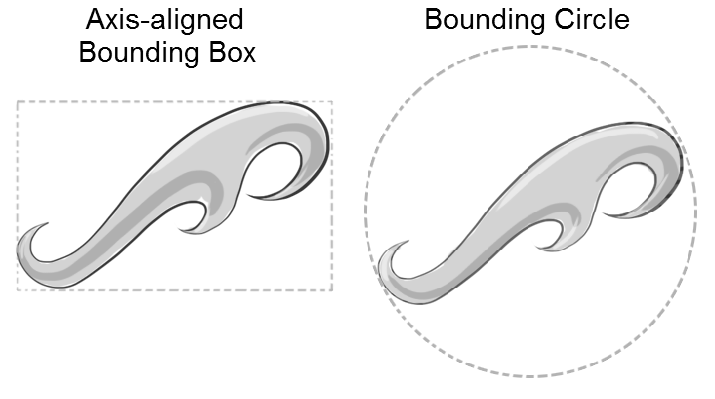
\includegraphics[width=0.7\linewidth]{images/chapter_navigazione_scena/box1.png}\hfill
 \caption[Bounding Box e Bounding Circle.]{Bounding Box e Bounding Circle.}
 \label{fig:navigazione_scena_navigator_oculus}
\end{figure}
\\
Per il presente lavoro di tesi è stato necessario utilizzare un tipo di volume di delimitazione che permettesse di ottenere un ottimo compromesso tra velocità di computazione e precisione di approssimazione dell’ oggetto contenuto.
\\
Nell’immagine è possibile osservare due efficienti tipologie di volumi di delimitazione che sono stati oggetto di studio al fine di valutare quello che meglio si addicesse per questo elaborato: \texttt{Bounding Box} e \texttt{Bounding Circle}.
\\
Nell’esempio la Bounding Box approssima meglio l’oggetto, non sempre però questo si verifica. 
Oggetti curvi infatti sono solitamente delimitati meglio da una Bounding Circle, mentre oggetti cubici vengono approssimati meglio da una Bounding Box.
\\
Per questo lavoro di tesi gli oggetti da inserire rappresentano per lo più mobili di arredamento, e solitamente questi difficilmente hanno una forma curvilinea. Gli studi effettuati hanno infatti permesso di verificare come uno o più oggetti di questo tipo fossero solitamente meglio delimitati da una Bounding Box.
\\
Inoltre le Bounding Box risultano più efficienti da calcolare rispetto alle Bounding Circle, quindi le prime sono state utilizzate durante la fase generale.
Inoltre esitono due differenti modalità di utilizzo delle bounding box: le \texttt{Axis-Aligned Bounding Box} (AABB) e le \texttt{Oriented Bounding Box} (OBB).
\begin{figure}[htb]
 \centering
 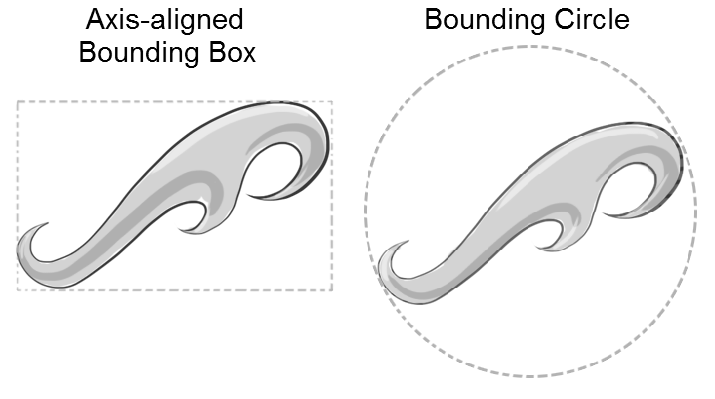
\includegraphics[width=0.7\linewidth]{images/chapter_navigazione_scena/box1.png}\hfill
 \caption[AABB e OBB.]{Le Axis-Aligned Bounding Box e le Oriented Bounding Circle.}
 \label{fig:navigazione_scena_navigator_oculus}
\end{figure}
\\
La AABB rappresenta una scatola rettangolare con sei facce dove ogni normale di faccia è sempre parallela con gli assi di riferimento del sistema di coordinate.
\\
Il vantaggio nell’utilizzo di questa notazione rappresenta la velocità di calcolo del volume di delimitazione. Esso viene infatti calcolato/rappresentato tramite due coordinate (x,y,z).
\\
La prima rappresenta il valore minimo di coordinata su ogni asse e cioè il minimo valore di x, y e z tra tutti i vertici dell’oggetto. La seconda rappresenta invece il valore massimo su ogni asse x,y,z tra tutti i vertici.
\\
Ulteriore vantaggio è la velocità di valutazione della collisione tra due AABB mediante un semplice controllo di sovrapposizione tra le due coordinate della prima Bounding Box e le due coordinate della seconda su ognuno dei tre assi.
\\

La OBB rappresenta, esattamente come la AABB, una scatola rettangolare con sei facce ma con un orientamento arbitrario.
\\
L’utilizzo di volumi OBB comporta notevoli miglioramenti nella delimitazione degli oggetti ruotati, portando alla generazione di meno spazio vuoto.
\\
A differenza delle AABB, la creazione di queste ed il test per l’intersezione risulta però estremamente complicato dal punto di vista delle operazioni algebriche da effettuare in quanto deve tenere conto dell’orientamento delle facce nelle tre dimensioni.
Nel presente lavoro di tesi è stato quindi utilizzato un volume di collisione di tipo AABB poco preciso ma molto performante.
\\
La precisione infatti non risulta importante durante la fase generale in quanto questo test preliminare permette solamente di individuare gli oggetti più probabile per la collisione ed a scartare dal calcolo di intersezione gli oggetti che sicuramente non collidono. Sarà poi la fase ristretta ad effettuare il calcolo più preciso, ma anche più dispendioso computazionalmente, sul sottoinsieme ottenuto dalla fase generale.
\\
La fase generale si basa sulla supposizione che se due volumi di delimitazione non collidono, allora anche gli oggetti al loro interno non possono collidere.
\\
Una metodologia comune per ottenere i volumi di delimitazione di oggetti complessi è quello di partizionare la scena in una rappresentazione gerarchica ad albero.
\\
Un albero in cui la radice rappresenta tutti gli oggetti presenti all’interno della scena ed ogni nodo contiene una piccola porzione di oggetti presenti in essa.
\\
Maggiore è il livello di profondità minore è la porzione di scena presa in considerazione.
La gerarchia generalmente viene modellata manualmente da un designer che conosce la scena. In questo lavoro di tesi era però fondamentale automatizzare il processo di generazione della gerarchia, rendendolo totalmente trasparente all’utente.
\\
Inoltre risultava essenziale che il processo di partizionamento potesse funzionare per ogni scena inserita all’interno del navigatore, indipendentemente da come essa fosse composta.
\\

Nella fase di partizionamento, viene suddiviso lo spazio 3D della scena in volumi di delimitazione sempre più piccoli. Questi volumi vengono organizzati secondo una gerarchia ad albero chiamata \texttt{Bounding Volume Hierarchy} (BVH) dove nelle foglie vengono inseriti gli oggetti presenti nella scena. 
Questi oggetti vengono poi raggruppati in piccoli insiemi diversi e racchiusi dentro un volume di delimitazione. Questi volumi sono a loro volta raggruppati in insiemi e racchiusi in volumi più grandi, questo procedimento continua in maniera ricorsiva fino a quando in cima all’albero non viene creata un volume che racchiude tutti gli oggetti presenti.
\\
L’albero creato permette di raggruppare all’interno di bounding box sottoinsiemi di oggetti che potrebbero collidere.
Ad esempio l’oggetto E potrebbe collidere con l’oggetto B, mentre è impossibile che possa collidere con l’oggetto A.
\begin{figure}[htb]
 \centering
 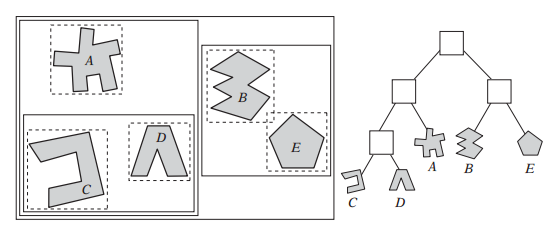
\includegraphics[width=1\linewidth]{images/chapter_navigazione_scena/partiz_tree.png}\hfill
 \caption[Bounding Volume Hierarchy.]{Bounding Volume Hierarchy.}
 \label{fig:navigazione_scena_partiz_tree}
\end{figure}
\\
L’algoritmo infatti individua che il padre della foglia dell’albero B è differente dal padre della foglia A, quindi è improbabile che possano collidere.
Questa fase permette quindi di scremare in maniera veloce tutte le collisioni che risultano improbabili.
\\
Nel presente lavoro di tesi è stato utilizzato questo albero per permettere un efficiente algoritmo di collisioni in una scena statica.
Nel contesto preso in esame, la scena infatti risulta immutabile nel tempo: sono totalmente assenti oggetti animati e quindi è impossibile che gli oggetti possano collidere tra loro.
Durante la navigazione in prima persona però l’osservatore è libero di muoversi all’interno dell’ambiente creato in Three.js.
\\
L’osservatore viene rappresentato come un oggetto inserito all’interno della scena a cui viene assegnato una propria BoundingBox di tipo AABB. 
Questo oggetto siccome in movimento può collidere con gli oggetti statici presenti nella scena.
Il calcolo di queste collisioni è essenziale ai fini di ricreare una passeggiata virtuale all’interno della scena, permettendo di camminare, saltare, salire e scendere scale. 
\\
Inoltre ha permesso di bloccare i movimenti di navigazione nel caso di attraversamento di oggetti o muri.
Il fatto che la scena sia statica permette di creare la gerarchia della scena una sola volta, in particolare solo quando viene avviata la navigazione in prima persona.
Calcolare più volte la gerarchia appesantirebbe inutilmente il ciclo di render in quanto l’albero ottenuto dai calcoli risulterebbe sempre identico.
\\
L’unico oggetto che varia è l’osservatore in quanto direttamente pilotato dall’utilizzatore del navigatore.

\begin{figure}[htb]
 \centering
 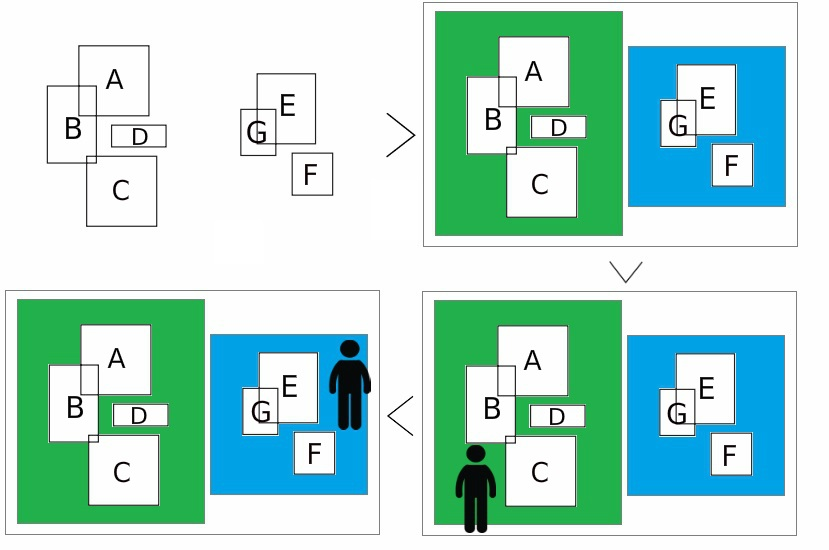
\includegraphics[width=1\linewidth]{images/chapter_navigazione_scena/partiz_oss.jpg}\hfill
 \caption[Il partizionamento nello spazio.]{Il partizionamento nello spazio.}
 \label{fig:navigazione_scena_partiz_oss}
\end{figure}

Nel dettaglio la scena creata in Three.js viene partizionata in volumi di delimitazione contenenti uno o più oggetti.
\\
Una volta calcolata la gerarchia viene valutato quale volume di delimitazione, tra quelli calcolati durante il partizionamento, contenga la  bounding box dell’oggetto che rappresenta l’osservatore.
\\
Questo calcolo viene effetuato ad ogni ciclo di render ma risulta estremamente veloce in quanto esegue un semplice test di appartenenza, non comportando quindi rallentamenti durante la renderizzazione.
\\
Una volta identificato il volume di delimitazione, gli oggetti presenti all’interno di esso vengono passati alla fase successiva. Tra tutti gli oggetti nella scena, quelli presenti all’interno del volume calcolato sono quelli hanno hanno maggiore probabilità di collidere con l’osservatore.
\\
Nella fase successiva viene valutato in maniera estremamente precisa se effettivamente la collisione è avvenuta.
\\
Nell’esempio visibile in figura, quando l’osservatore si trova all’interno della bounding box colorata di verde può collidere solamente con i quattro oggetti A,B, C e D. Quindi solamente questi oggetti verrano valutati nella fase successiva mentre gli altri saranno scartati.
Quando invece si trova nella bounding box blu, gli oggetti che passano nella fase successiva sono E, F e G, mentre gli altri sono scartati.
\\
Questo algoritmo permette di ottenere ottime prestazione quando la scena è costituita da un alto numero di oggetti, come le scene di interni prese in esame in questo elaborato.
Nel presente lavoro di tesi infatti ha permesso, in scene costituite da centinaia di oggetti, di valutare ad ogni ciclo di render solamente un manciata di oggetti e di ignorare completamente gli altri in quanto troppo lontani per potere collidere con l’osservatore virtuale.
\\
I dettagli implementati di questa soluzione veranno esaminati nel paragrago \ref{sec:chapter_navigazione_scena_implementazione}.

\subsection{Fase ristretta}

La fase ristretta ha il compito di calcolare in maniera esatta la collisione tra due o più oggetti. Il sottoinsieme di oggetti che potenzialmente potrebbero collidere, calcolato durante la fase generale, viene utilizzato in questa fase  al fine di valutare se effettivamente la collisione è avvenuta o meno.
\\
Inoltre, durante questa fase, viene calcolato il punto di contatto in cui la collisione è avvenuta, permettendo la gestione di differenti casi di collisione.
\\
Nel dettaglio, per calcolare con estrema precisione delle collisioni avvenute tra l’osservatore con la scena statica, è stato utilizzato un algoritmo di \texttt{ray casting} specifico per la gestioni delle collisioni.
Questo tipo di algoritmo risulta particolarmente efficiente e permette di migliorare notevolmente le prestazioni di rendering durante la navigazione.
\\
Durante l’algoritmo di ray casting vengono lanciati dei raggi, rappresentati tramite vettori, a partire dall’origine dell’Object 3D (l’osservatore) verso differenti direzioni nello spazio.
\\
Se il raggio lanciato colpisce un oggetto e quest’ultimo si trova ad una distanza ravvicinata (all’interno di un intervallo specifico di collisione) dall’osservatore, allora i due collidono.
In questo lavoro di tesi, l’algoritmo di Ray Tracing è stato opportunamente implementato e parametrizzato al fine di ottenere un ottimo compromesso tra velocità di navigazione in prima persona  e precisione nel riconoscimento delle collisioni.
\\
Nel dettaglio la tecnica del Ray Tracing se non gestita correttamente può rallentare le prestazioni di rendering, rendendo impossibile l’utilizzo del navigatore in ambiente web, anche su hardware poco performanti.
\\
In particolare durante il lavoro di tesi sono stati inizialmente individuati i fattori che maggiormente incidessero sulle performance dell’algoritmo, e successivamente è stata creata una metodologia efficiente e precisa per la collision detection.
I fattori che inficiano maggiormente sono:
\begin{itemize}
\item Il numero dei raggi lanciati nella scena ad ogni ciclo di render.
\item Il punto di partenza e la direzione in cui vengono lanciati i raggi.
\item Il numero di oggetti da valutare per ogni raggio lanciato.
\item La distanza minima a cui deve trovarsi il primo oggetto intersecato dal raggio rispetto all’osservatore per permettere l’identificazione della collisione.
\item La forma dell’oggetto che viene intersecato dal raggio.
\end{itemize}

Ogni fattore sopra descritto è stato studiato approfonditamente ed accompagnato da varie sperimentazioni su scene di media e grandi dimensioni.
\\
Nel dettaglio, per la realizzazione di questo algoritmo, si è seguito un approccio iterativo incrementale guidato dai test, che è passato attraverso varie iterazioni.
Scegliere il numero di raggi da lanciare a partire dall’origine dell’osservatore è stato fondamentale. Risulta infatti essenziale lanciare un raggio in ogni direzione in cui l’osservatore è in grado di muoversi.
\\
Questo permette di bloccare la direzione di movimento dell’osservatore in cui è presente l’ostacolo con cui esso collide.
\\
La collisione avviene solamente se il raggio colpisce l’oggetto, ed il punto intersecato si trova ad una distanza dall’osservatore in un intervallo compreso tra 0 e 20 cm. 
Questo intervallo di tolleranza è stato ottenuto in seguito a sperimentazioni ed ha permesso di il riconoscimento di ostacoli con elevata precisioni.
\\
Nel dettaglio l’osservatore, esattamente come una persona reale, può muoversi in 8 direzioni: avanti, indietro, a destra, a sinistra e le 4 direzione oblique.
\\
Ad ogni direzione di movimento viene associato un diverso vettore nella stessa direzione.
Per semplicità di trattazione, viene ora supposto che i vettori lanciati siano perpendicolari all’osservatore e paralleli al piano in cui si muove. Verrà spiegato successivamente come questo non sia però sufficiente per la creazione di un algoritmo preciso di collisione.
\newpage
\begin{figure}[htb]
 \centering
 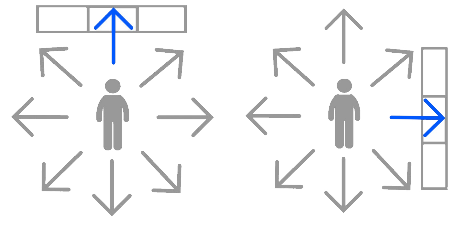
\includegraphics[width=0.8\linewidth]{images/chapter_navigazione_scena/collisioni1.png}\hfill
 \caption[Esempio di collisione.]{Scena vista dall'alto. Esempio di collisione.}
 \label{fig:navigazione_scena_collisioni1}
\end{figure}
Nell’esempio in figura \ref{fig:navigazione_scena_collisioni1}  viene rappresentato l’osservatore visto dall’alto con gli otto vettori direzionati nelle otto direzioni principali di movimento.
\\
Nell’immagine a sinistra il vettore frontale interseca il muro, questo permette di impedire il movimento in avanti. L’osservatore in questo modo non attraversa il muro, rimanendo bloccato da esso.
\\
Nell’immagine a destra invece il vettore laterale destro interseca con il muro, impedendo in questo modo il movimento verso la direzione laterale destra.
Quindi ogni volta che un vettore associato ad una direzione di movimento individua un ostacolo, il movimento in quella direzione viene impedito.
\\
Risulta quindi fondamentale che questi vettori ruotino insieme all’osservatore. In particolare i vettori devono ruotare insieme all’asse di rotazione verticale dell’osservatore, solitamente l’asse y se la superficie si trova sul piano orizzontale x,z.
\begin{figure}[htb]
 \centering
 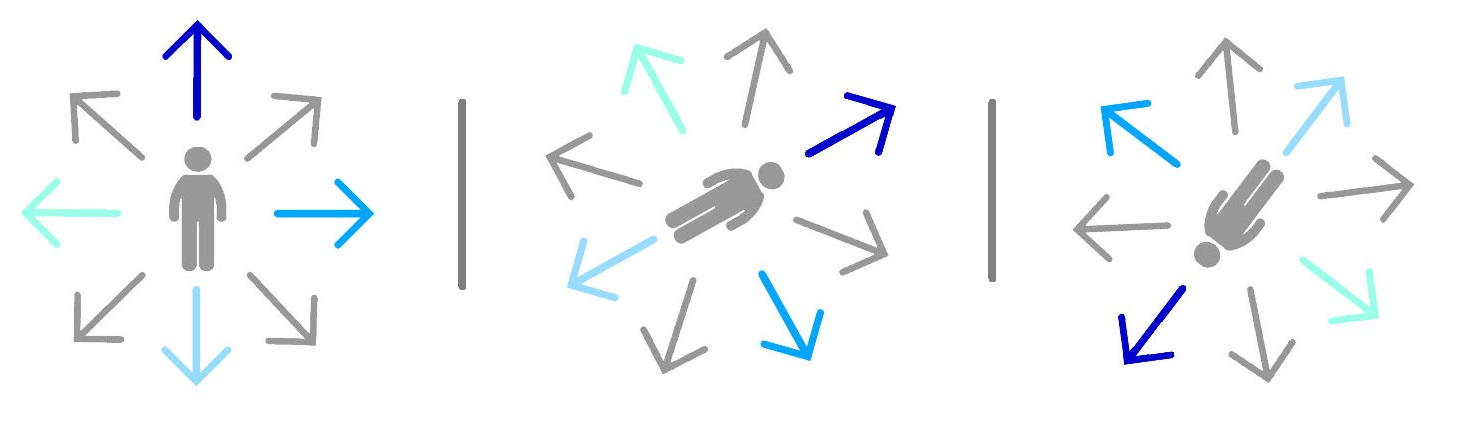
\includegraphics[width=1\linewidth]{images/chapter_navigazione_scena/coll_rotat.jpg}\hfill
 \caption[Veduta dall'alto dei vettori dell'osservatore.]{La rotazione dei vettori associati all'osservatore.}
 \label{fig:navigazione_scena_coll_rotat}
\end{figure}
\\
Questi otto vettori risultano quindi fondamentali al fine di individuare all’interno della scena virtuale oggetti con cui l’osservatore può collidere.
\\
Essi però non possono essere lanciati perpendicolarmente all’osservatore e paralleli rispetto al piano in cui si muove in quanto, con una elevata probabibilità, non intersecherebbero oggetti con forme convesse come tavolini.
\\
I raggi infatti, molto probabilmente, non colpirebbero il tavolino in quanto lanciati nella zona vuota sopra o sotto di esso (figura \ref{fig:navigazione_scena_collision_tav1}).
\begin{figure}[htb]
 \centering
 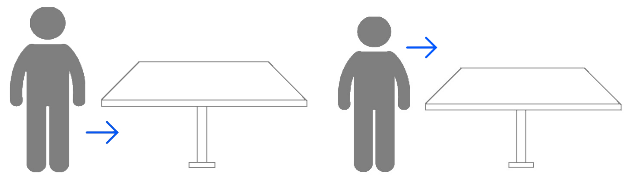
\includegraphics[width=1\linewidth]{images/chapter_navigazione_scena/collision_tav1.png}\hfill
 \caption[Raggi su oggetti convessi.]{Intersezione dei raggi su oggetti convessi.}
 \label{fig:navigazione_scena_collision_tav1}
\end{figure}
\\
Una possibile metodologia per la risoluzione di questo inconveniente è quella di considerare gli oggetti tramite la loro Bounding box e di lanciare i raggi a partire dal basso dell’osservatore virtuale (i piedi dell’osservatore virtuale).
\begin{figure}[htb]
 \centering
 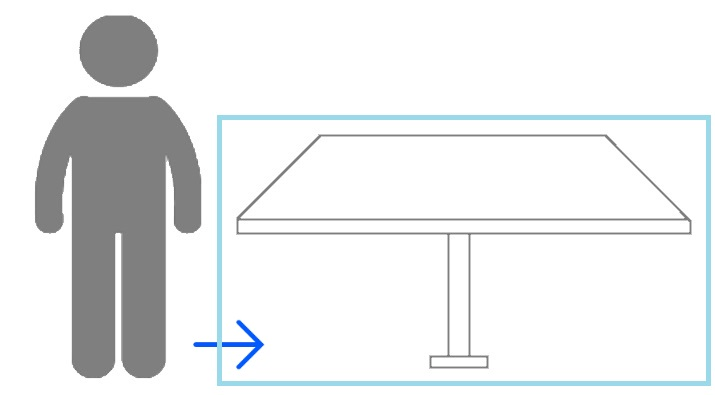
\includegraphics[width=0.6\linewidth]{images/chapter_navigazione_scena/collision_tav2.jpg}\hfill
 \caption[Raggi sulle Bounding Box.]{Intersezione dei raggi sulle Bounding Box degli oggetti convessi}
 \label{fig:navigazione_scena_collision_tav2}
\end{figure}
\\
Se infatti i raggi vengono lanciati da una altezza bassa, vicina alla superficie che sorregge l’osservatore, allora certamente colpiranno la Bounding Box che racchiude l’oggetto della scena. Se invece i raggi vengono lanciati da un punto elevato allora avranno una bassa probabilità di intersecare il volume di delimitazione, non permettendo quindi il riconoscimento della collisione.
\\
Utilizzare le Bounding Box permette di risolvere questo problema ma comporta, per particolari geometrie di oggetti, un problema non indifferente: il rischio di collisione in punti in cui non si dovrebbe. Valutare le collisioni con questi volumi comporta di fatto una notevole diminuzione dello spazio di movimento dell’osservatore.
\begin{figure}[htb]
 \centering
 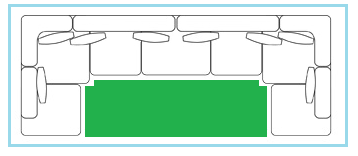
\includegraphics[width=0.7\linewidth]{images/chapter_navigazione_scena/divano.png}\hfill
 \caption[Problemi utilizzo Bounding Box.]{Bounding Box che non delimita perfettamente il volume del divano}
 \label{fig:navigazione_scena_divano}
\end{figure}
\\
Nell’immagine di esempio è possibile notare come la Bounding Box non permetta di delimitare perfettamente il volume del divano.
\\
Siccome i raggi lanciati collidono con la Bounding Box invece che con l’oggetto, l’algortimo non permette all’osservatore di entrare all’interno della zona segnata in verde. Zona che di fatto dovrebbe essere invece accessibile.
\\
Questa imprecisione soprattutto in piccole abitazioni, comporta problemi non indifferenti durante la navigazione, impedendola in alcuni casi.
\\
Inoltre in questo lavoro di tesi è risultato fondamentale ottenere l’algoritmo di collisione più preciso possibile in ambienti web, per questo motivo la Bounding Box è stata abbandonata in favore di una tecnica differente.
\\
Gli otto vettori vengono sempre lanciati ad una altezza bassa dell’osservatore ma vengono inclinati verso l’alto. Questo permette il riconoscimento di tutti gli oggetti convessi in maniera estremamente precisa. L’altezza da cui vengono lanciati viene esaminata quando verrano descritti i vettori che permettono di salire/scendere le scale.
\\
L’angolo con cui vengono inclinati questi raggi è stato oggetto di studio e sperimentazione, 
Gli angoli di inclinazione verso l’alto dei vettori associati alle quattro direzioni principali risultano di 65 gradi, mentre quelli delle quattro direzioni oblique risultano di circa 80 gradi.
\\
\begin{figure}[htb]
 \centering
 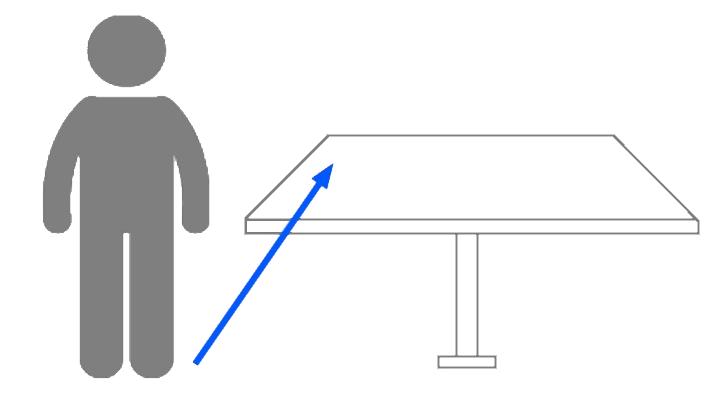
\includegraphics[width=0.7\linewidth]{images/chapter_navigazione_scena/collision_tav3.jpg}\hfill
 \caption[Raggi inclinati verso l'alto.]{Raggio dell'osservatore inclinato verso l'alto.}
 \label{fig:navigazione_scena_collision_tav3}
\end{figure}
\\
Quando l’osservatore collide un oggetto e si muove in una delle quattro direzioni principali (aventi, indietro,destra,sinistra), l’unico vettore ad intersecare è proprio quello associato alla direzione principale di movimento in quanto meno inclinato.
\\
Il movimento in quella direzione risulta impedito mentre i movimenti nelle direzioni oblique risultano ancora possibili in quanto i raggi associati non sono stati intersecati dall’oggetto perché più inclinati verso l’alto.
\\
Utilizzare invece per tutti gli otto vettori la stessa inclinazioni, nella maggior parte delle situazioni, non avrebbe permesso il movimento nelle direzioni oblique. 
Questo perché nella maggior parte dei casi sia il raggio nelle direzione principale di movimento, sia i due raggi obliqui vicini ad esso verrebbero intersecati dall’oggetto all’interno dell’intervallo di distanza (0-20 cm).
\\
Inoltre risultava fondamentale mantenere la distanza massima di collisione a 20 cm per permettere un tipo di collisione credibile con l’oggetto intersecato. Quando infatti una persona collide con un muro si ferma a qualche cm prima di toccarlo, questo intervallo permette di ricreare virtualmente questo comportamento reale.
\\
L’utilizzo di due differenti angolazioni ha permesso quindi di utilizzare l’intervallo di distanza di collisione ed ha permesso di ricreare un tipo di navigazione fluida in tutte le direzioni, riproducendo molto fedelmente una camminata nel mondo reale.
\\

Oltre a questi otto vettori ne vengono utilizzati altri cinque:
\begin{itemize}
\item Quattro vettori permettono il riconoscimento di oggetti su cui è possibile salire come ad esempio le scale.
\item Un vettore permette il riconoscimento del piano su cui l’osservatore è poggiato, permettendo in questo modo all’osservatore di rimanerci sopra.
\end{itemize}
I quattro vettori sono direzionati in avanti, indietro, a destra ed a sinistra ma questa volta inclinati verso il basso. Sperimentazioni svolte hanno confermato che per il riconoscimento di oggetti su cui è possibile salire sono sufficiente quattro vettori invece che otto, permettendo di migliorare l’efficienza dell’algoritmo.
\\
Questi quattro vettori sono lanciati verso il basso con un angolo di inclinazione di 57 gradi, scelto in base ad opportune prove, a partire da uno specifico punto dell’altezza dell’osservatore. Questo punto viene calcolato in base a quanto è alto l’osservatore virtuale; tutti e 13 i raggi vengono lanciati dal 15\% dell’altezza dell’osservatore.
\\
Quindi supponendo l’osservatore alto 1.80 m, non solo i quattro raggi direzionati verso il basso, ma anche gli otto verso l’alto saranno lanciati a partire da una altezza di 27 cm.
Questo vuol dire che l’osservatore virtuale al massimo sarà in grado di salire gradini alti 27 cm.
\begin{figure}[htb]
 \centering
 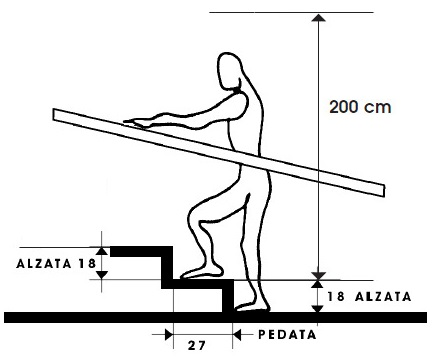
\includegraphics[width=0.7\linewidth]{images/chapter_navigazione_scena/scala.jpg}\hfill
 \caption[Dimensioni di una scala da interno.]{Dimensioni di una scala da interno.}
 \label{fig:navigazione_scena_collision_scala}
\end{figure}
\\
Normalmente i gradini hanno una alzata (altezza) compresa tra i 17 ed i 20 cm \cite{scale_pedata}.
I raggi inviati verso il basso dall’algoritmo permettono di salire su questo tipo di scale, inoltre permettono anche, in base all’altezza dell’osservatore, di salire gradini più alti. 
Questo per consentire una navigazione fluida anche in ambienti in cui le scale sono particolarmente ripide o in cui sono presenti salite molto pendenti.
\\ 
L’algoritmo creato permette infatti di salire agevolmente le comuni scale da abitazioni con pendenza compresa tra i 20 ed i 45 gradi, ma anche di salire scale particolarmente ripide con pendenza fino a 60 gradi, utilizzate soprattutto all’interno di locali tecnici \cite{scale_gradi}.
\\
La pedata, cioè la profondità del gradino, non deve essere riconosciuta in quanto l’algoritmo permette all’osservatore di rimanere sopra una superficie piana, qualunque sia la grandezza di essa. Il piano che lo sorregge viene valutato dal vettore lanciato verso il basso.
\\
Questo vettore direzionato verso il basso, entra perpendicolarmente al piano su cui è poggiato l’osservatore. Esso riconosce il piano su cui è poggiato l’osservatore  e permette ad esso di rimanere ancorato sopra la superficie.
\\
La collisione avviene se il raggio interseca una superficie che si trova ai piedi dell’osservatore (all’altezza zero); anche in questo caso è presente una soglia di tolleranza di intersezione.
\\ 
Se la collisione avviene allora l’osservatore rimane poggiato sopra l’oggetto con cui ha intersecato.
\\
Se invece la collisione non avviene allora l’osservatore cade in direzione verticale perpendicolare al piano e diretta verso il basso fino a quando il vettore non interseca con una superficie. La velocità con cui cade l’osservatore virtuale, esattamente come nella vita reale, dipende dall’ accelerazione di gravità: $g = 9,8 \frac{m}{s^2}$
\\
Il corpo che cade si muove quindi con un moto rettilineo uniformemente accelerato in quanto viene supposto che non ci sia attrito dovuto dall’aria.
Questo vettore è stato inoltre fondamentale per simulare virtualmente il movimento del salto.
In figura è possibile osservare da una veduta laterale le angolazioni dei vettori principali utilizzati.
\\
Di fatto quindi l’utilizzo di soli 13 vettori ha permesso di creare una metodologia di collision detection precisa e, grazie al basso numero di raggi utilizzato, efficiente.
\\
Efficiente anche perché ogni raggio viene valutato sul piccolo sottoinsieme degli oggetti con cui l’osservatore ha la più alta probabilità di collisione, calcolati durante la fase generale.
\\
Questa metodologia si adatta ad ogni scena creabile tramite l’editor, rendendo trasparente all’utente tutta la tecnologia su cui è basata la navigazione della scena.
\begin{figure}[htb]
 \centering
 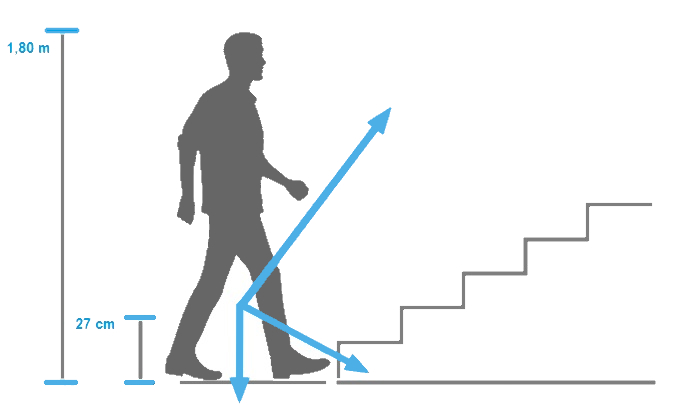
\includegraphics[width=0.9\linewidth]{images/chapter_navigazione_scena/collision_gradini.jpg}\hfill
 \caption[I raggi che permetto di salire.]{I raggi che permettono di salire e scendere scale.}
 \label{fig:navigazione_scena_collision_gradini}
\end{figure}
